\documentclass[10pt,twocolumn,twoside]{genpaper}
\usepackage[numbers,sort&compress]{natbib}

\newcommand{\npscarf}{$\mathtt{npScarf}$}
\newcommand{\npscarfg}{$\mathtt{npScarf\_wag}$}
\newcommand{\npreader}{$\mathtt{npReader}$}
\newcommand{\npanalysis}{$\mathtt{npAnalysis}$}
\newcommand{\npbarcode}{$\mathtt{npBarcode}$}
\newcommand{\npgraph}{$\mathtt{npGraph}$}
\newcommand{\canu}{$\mathtt{Canu}$}
\newcommand{\unicycler}{$\mathtt{Unicycler}$}
\newcommand{\spades}{$\mathtt{SPAdes}$}
\newcommand{\hspades}{$\mathtt{hybridSPAdes}$}
\newcommand{\albacore}{$\mathtt{Albacore}$}
\newcommand{\racon}{$\mathtt{Racon}$}
\newcommand{\metrichor}{$\mathtt{Metrichor}$}
\newcommand{\minimap}{$\mathtt{minimap2}$}
\newcommand{\miniasm}{$\mathtt{miniasm}$}
\newcommand{\bwa}{$\mathtt{BWA\text{-}MEM}$}

\newcommand{\ec}{\emph{E.~coli}}
\newcommand{\sce}{\emph{S.~cerevisae}}
\newcommand{\kp}{\emph{K.~pneumoniae}} 

\newcommand{\IE}{\emph{i.e.}}
\newcommand{\EG}{\emph{e.g.}}
\newcommand{\review}[1]{\textcolor{red}{#1}}

\newcommand{\cthead}[2]{\multicolumn{#1}{c}{\textbf{#2}}}
\definecolor{Gray}{gray}{0.9}
\newcommand{\cir}{$^\ast$}
\newcommand{\bres}[1]{{\bf #1}}

\usepackage{pdfpages} 
\usepackage{mathtools}
\usepackage{play}
\usepackage{makeidx}
\usepackage{xcolor,colortbl}
\usepackage{longtable}
\usepackage{booktabs}
\usepackage{hyperref}
\usepackage{pdflscape}

\usepackage{amsmath,amsfonts,amssymb} % this is handy for mathematicians and physicists
			      % see http://www.ams.org/tex/amslatex.html

% \usepackage{showkeys} % this shows what labels you are using for cross
		      % references

\usepackage{graphicx} % standard graphics package for inclusion of
		      % images and eps files into LaTeX document

\usepackage{multirow} 

\usepackage{float}
\usepackage[caption = false]{subfig}
% this code hacked from that of R Chandrasekhar from UWA
\newif\ifpdf
\ifx\pdfoutput\undefined
	\pdffalse    % we are not running pdfLaTeX
\else
	\pdfoutput=1 % we are running pdfLaTeX
	\pdftrue
\fi

\ifpdf
	\DeclareGraphicsExtensions{.pdf}  % this command defined in graphicx
	\pdfcompresslevel=9  % 0: no compression, 9: highest compression
			     % or, set compress_level 9 in file pdftex.cfg
\else
	\DeclareGraphicsExtensions{.ps}
\fi

\usepackage[linesnumbered,boxed,ruled,vlined]{algorithm2e}
\newcommand\mycommfont[1]{\footnotesize\ttfamily\textcolor{blue}{#1}}
\SetCommentSty{mycommfont}
% For code embedding (Bash, Java...)
\usepackage{listings}
\lstset{basicstyle=\ttfamily,
  showstringspaces=false,
  commentstyle=\color{red},
  keywordstyle=\color{blue}
}
\usepackage{latexsym}
\usepackage{mathtools}
\usepackage{amsmath}
\DeclareMathOperator*{\argmax}{argmax}
\DeclareMathOperator*{\argmin}{argmin}

\usepackage{xr}
\externaldocument{supplementary}
%%%%%%%%%%%%%%%%%%%%%%%%%%%%%%%%%%%%%%%%%%%%%%%%%%%%%%%%%%%%%%%%%%%%%%%%%%%%%%
%%%%%%%%%%%%%%%%%%%%%%%%%%%%%%%%%%%%%%%%%%%%%%%%%%%%%%%%%%%%%%%%%%%%%%%%%%%%%%
%% Some functions provided  by the class

%Display line numbers on the margins
\lineno

%% use \onecolumn for onecolumn paper
\onecolumn

\title{Real-time resolving assembly graph by ONT long reads data}
\shorttitle{Real-time Scaffolding with Assembly graph}

%Authors
\author[1,$\ast$]{Son Hoang Nguyen}
\author[2]{Minh Duc Cao}
\author[1,$\ast$]{Lachlan Coin}

%Affiliation
\affil[1]{Institute for Molecular Bioscience, the University of Queensland, 
St Lucia, Brisbane, QLD 4072 Australia}
\affil[2]{4catalyzer}
\correspondingauthor{
\textsuperscript{$\ast$}
To whom correspondence should be addressed. 
E-mails: l.coin@imb.uq.edu.au,s.hoangnguyen@imb.uq.edu.au
}

%Display ``This manuscript was compiled on XXXX''
\compiledate

%Set abstract (see below)
\abstract{
A real-time assembly pipeline for Oxford Nanopore Technology (ONT) data is important for either saving sequencing resources or reducing turnaround time for data analyses. The previous approach from \npscarf{} provided a fast-response streaming algorithm for such task but was relatively prone to mis-assemblies compared to other graph-based methods. 
Here we present \npgraph{}, a real-time hybrid assembly software using the assembly graph instead of the separated pre-assembly contigs. It is able to produce more complete genome assembly by resolving the path finding problem on the assembly graph using long reads as the traversing guide. 
The application on synthetic and real data set of isolate genomes show improved accuracy while still maintaining the required computational cost extremely low. 
%On top of that, we apply \npgraph{} on mock community in the very first application to improve metagenomics assembly in real-time with nanopore data. 
With \npscarf{}, the built-in graphical user interface (GUI) can provide users a comprehensive look-and-feel of the whole assembly process. The tool and source code is available at \url{https://github.com/hsnguyen/assembly}.
} 
%Set keywords
\keywords{hybrid assembly, assembly graph, real-time analysis, nanopore sequencing}

%%%%%%%%%%%%%%%%%%%%%%%%%%%%%%%%%%%%%%%%%%%%%%%%%%%%%%%%%%%%%%%%%%%%%%%%%%%%%%

\begin{document}
%Abstract and keywords have to be defined before \maketitle
\maketitle
\thispagestyle{fancy}

%%%%%%%%%%%%%%%%%%%%%%%%%%%%%%%%%%%%%%%%%%%%%%%%%%%%%%%%%%%%%%%%%%%%%%%%%%%%%%%%%%%
\section*{Introduction}
% \begin{itemize}
% \item The importance of having a real-time assembler for bacterial and small genomes: e.g. npscarf 
% \item The difficulty to resolve assembly graph in real-time.
% \item Available hybrid assembly methods using long reads: unicycler, ...
% \item an online algorithm to resolve assembly graph by long reads is needed, ...
% \item Requirements
%     \begin{itemize}
%     \item Support streaming: efficient with high yield (armortized analysis)
%     \item Statistically robust: online modification of the dynamic graph, back tracking edge deletion...
%     \item Standardisation : output GFA in real-time
%     \end{itemize}
% \end{itemize}
Streaming assembly methods had been proven to be useful in saving time and resources compared to the conventional batch algorithms with examples included \EG{} $\mathtt{Faucet}$~\cite{Rozov2017faucet} and \npscarf{}~\cite{Cao2017scaffolding}. The first method allows the assembly graph to be constructed incrementally as long as reads are retrieved and processed. This practice is helpful dealing with huge short-read data set because it can significantly reduce the local storage for the reads, as well as save time for a De Bruijn graph (DBG) construction while waiting for the data being retrieved.
\npscarf{}, on the other hand, is a hybrid assembler working on a pre-assembly set of short-read assembly contigs. It functions by scaffolding the contigs using nanopore sequencing which is well-known by the real-time property. The completion of genome assembly in parallel with the sequencing run provides explicit benefits in term of resource control and turn-around time for analysis~\cite{Cao2017scaffolding}.  

% Why hybrid???
Hybrd approaches are still common practice in genome assembly and data analyses when Illumina sequencing remains the most favoured option in terms of cost and accuracy to date.
On the other hand, the third-generation sequencing methods such as Pacbio or Oxford Nanopore Technology are well-known for the ability to produce much longer reads that can further complete the Illumina assembly.
As the consequence, it is rational to combine two sources of data together in a hybrid method that can offer accurate and comptete genomes at the same time.
\npscarf{}, following that philosophy, had been developed and deployed on real microbial genomes.

However, due to the greedy bridging approach of the contigs-based streaming algorithm, \npscarf{}`s results might suffer from mis-assemblies~\cite{Wick2017unicycler,Giordano2017}. 
A default setting were optimzed for microbial genomes input but cannot fit for all data from various experiments in practice.
Also, the gap filling step has to rely on the low quality nanopore reads thus the accuracy of the final assembly is affected as well. 
To tackle the quality issue while maintaining its streaming feature, a bridging method by assembly graph traversing is proposed. 
In which, after the construction of a compact DBG assembly graph, the next step is to traverse the graph, resolve the repeats and identify the longest possible un-branched paths that would represents contigs for the final assembly.

Hybrid assembler using nanopore data to resolve the graph has been implemented in $\mathtt{hybridSPAdes}$ \cite{AntipovKM2015} or \unicycler{} \cite{Wick2017unicycler}. 
In general, the available tools employ batch-mode algorithms on the whole long-read data set to generate the final genome assembly. 
In which, the \spades{} hybrid assembly module, from its first step, exhaustively looks for the most likely paths (with mininum edit distance) on the graph for each of the long read given but only ones supported by at least two reads are attained. In the next step, these paths will be subjected to a decision-rule algorithm, namely $\mathtt{exSPAnder}$~\cite{Prjibelski2014}, for repeat resolution by step-by-step expansion, before output the final assembly.
On the other hand, \unicycler{}'s hybrid assembler will initially generate a consensus long read for each of the bridge from the batch data. 
The higher quality consensus reads are used to align with the assembly graph to find the best paths bridging pairs of anchored contigs.
While the latter method employs the completeness of the data  set from the very beginning for a consensus step, the former only iterates over the batch of possible paths and relies on a scoring system for the final decision of graph traversal. For that reason, the first direction is more suitable for a real-time pipeline.
    
Nonetheless, the challenge to adapt this approach into a real-time mechanism is obvious, mainly from building a progressive implementation for path-finding and graph reducing module which are essential for a streaming graph assembler. 
To achieve that, we apply a modified DFS (depth-first search) mechanism and a dynamic voting algorithm into an on-the-fly graph resolver.
The method is implemented in \npgraph{}, a user-friendly tool with GUI that can traverse the assembly graph and bridge its components in real-time as long as the nanopore sequencing process is still running. 
 
We use different hybrid data sets to study the \npgraph{}`s performance and compare with other available tools with similar functionality, such as \npscarf{}, \unicycler{} and \hspades{}. Even though all data were from microbial genomes, the complexity of the input graphs range from few hundred to ten thousands of components, synthesized \emph{in silico} or sequenced from \emph{in vitro} samples.
%Particularly, for the first time, we employ a pipeline in an attempt to complete metagenomics assembly in real-time. 
%We aim to develop a simple approach on top of \npgraph{} to adapt with metagenomics while minimizing additional processing steps. In fact, only one more step for population binning is needed to make \npgraph{} functions on genomes of a mock community.
%Despite a rather straightforward methodology, the pipeline has shown consecutively enhanced assembly from the fragmented short-read DBG graph.
%%%%%%%%%%%%%%%%%%%%%%%%%%%%%%%%%%%%%%%%%%%%%%%%%%%%%%%%%%%%%%%%%%%%%%%%%%%%%%%%%%%
\section*{Results}
\subsection*{\npgraph{} -- a tool to resolve assembly graph in real-time}
\npgraph{}'s input consists of Illumina assembly graph resulted from running assembler, e.g. \spades{}~\cite{BankevichNA2012}, $\mathtt{Velvet}$ \cite{Zerbino2008}, $\mathtt{AbySS}$ \cite{Simpson2009} on Illumina short reads, together with long reads from third generation sequencing technology (Oxford Nanopore Technology, Pacbio).
The long reads will be aligned with the contigs in the assembly graph to indicate longer paths that should be traversed. These local paths, given sufficient data, are expected to untangle the complicated graph and guide to the global Eulerian paths (or cycles if possible) that represent the entire genomic sequences. 
\npgraph{} can be invoked and fully function from the command-line interface. In addition, in order to aid the visualization of the assembly process, a GUI has been developed as well.

\begin{figure}[!hpt]
\centering
\parbox{\textwidth}{
    \parbox{.57\textwidth}{
        \subfloat{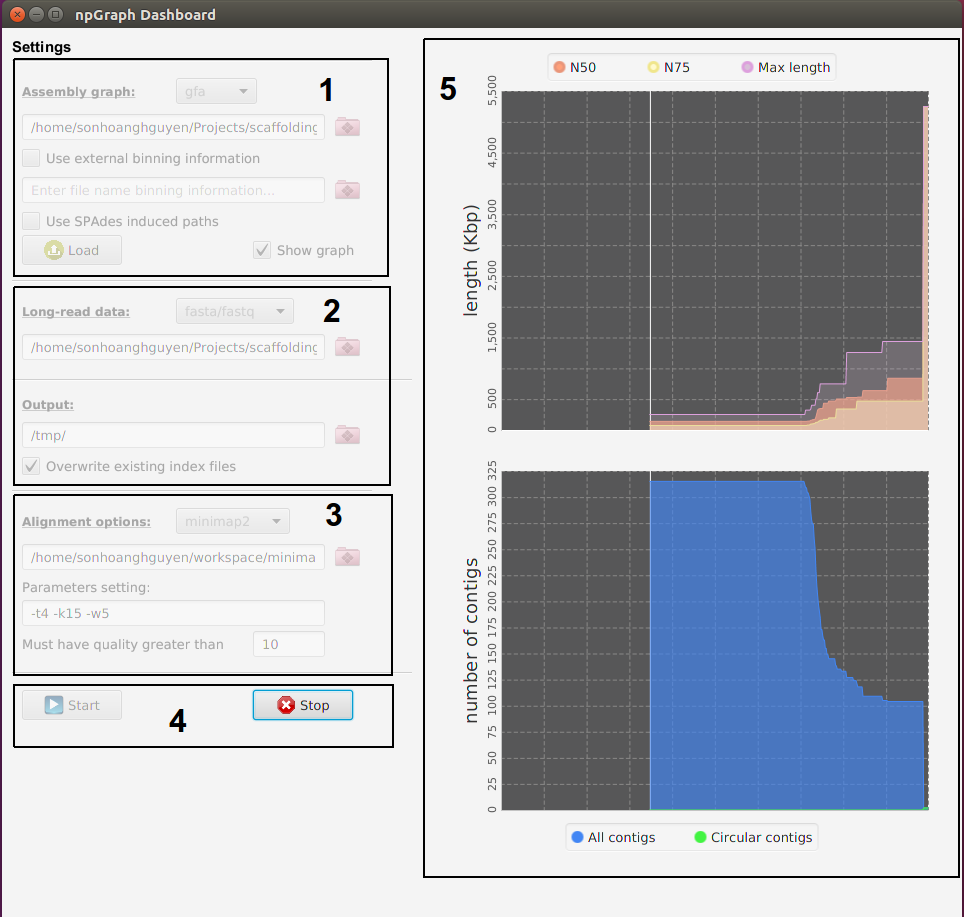
\includegraphics[width=\hsize]{images/dashboard.png}}
    }
    \hskip1em
    \parbox{.44\textwidth}{%
        \subfloat{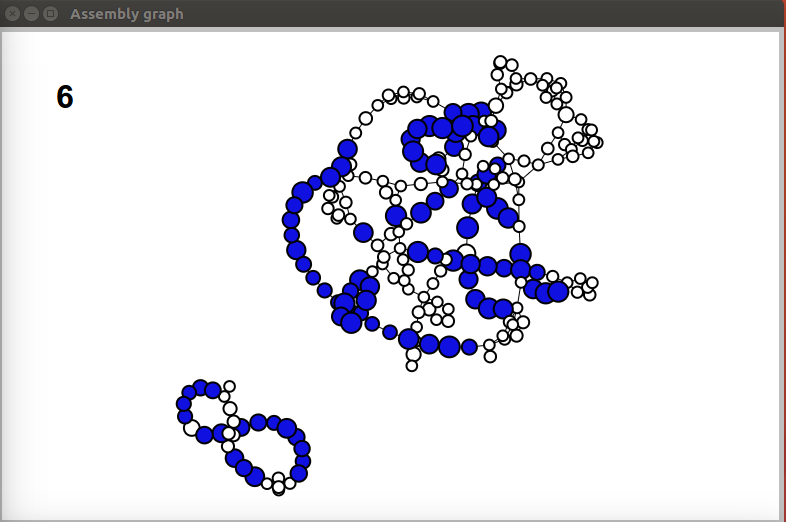
\includegraphics[width=\hsize]{images/graph-view.png}}
        \vskip1em
        \subfloat{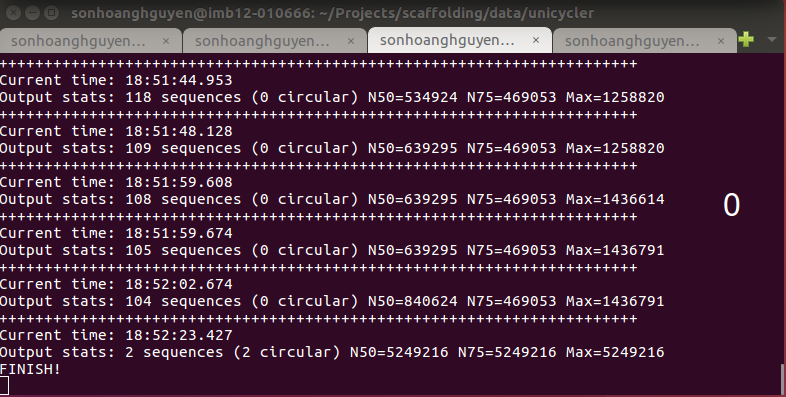
\includegraphics[width=\hsize]{images/console-view.png}}  
    }
}
\caption[\npgraph{} user interface]{\npgraph{} user interface including Console (\textbf{0}) and GUI components (\textbf{1}-\textbf{6}). The GUI consists of the Dashboard (\textbf{1}-\textbf{5}) and the Graph View (\textbf{6}). From the Dashboard there are 5 components as follow: \textbf{1} the assembly graph input field; \textbf{2} the long reads input field; \textbf{3} the aligner settings field; \textbf{4} control buttons (start/stop) to monitor the real-time scaffolding process; \textbf{5} the statistics plots for the assembly result.}
\label{figure:npgraph_gui}
\end{figure}

The GUI includes the dashboard for control the settings of the program and another pop-up window for a simple visualization of the assembly graph in real-time (Figure~\ref{figure:npgraph_gui}).
In this interface, the assembly graph loading stage is separated from the actual assembly process so that users can check for the graph quality first before carry out any further tasks. The box numbered \textbf{1} on Figure~\ref{figure:npgraph_gui} is designed for this task.
Only after an assembly graph is loaded successfully, users can move to box \textbf{2} to specify the nanopore input data.
Settings for an aligner (\bwa{} or \minimap{}) in box \textbf{3} is required if the input is the raw sequences in FASTA/FASTQ format. Another option is to run the alignment independently and provide SAM/BAM input for the next stage of bridging and assembly. This stage is controlled by buttons in box \textbf{4}: the START button ignites the process while the STOP button can prematurely terminate it and output the assembly result till that moment. The plots from the right panel (\textbf{5}) depicts real-time statistics of the assembly contigs inferred from the graph.
From the second window (\textbf{6}), the colored vertices imply unique contigs while the white ones involve either unspecified or repetitive elements. The number of different colors (other than white) indicates the amount of abundant groups being detected as population bins (\EG{} chromosome versus different plasmids, or different bins in metagenomics).

A proper combination of command line and GUI can provide an useful streaming pipeline that copes well with MinION output data. The practice is similar to the previous developed pipelines~\cite{CaoGC2016,Cao2017scaffolding,Nguyen2017barcode} that allow the analysis to take place abreast to a nanopore sequencing run.

\subsection*{Evaluation using synthetic data}
To evaluate the performance of the method, \npgraph{} was tested along with \spades{}, its hybrid assembly module~\cite{AntipovKM2015}, \npscarf{}, and Unicycler version 0.4.6 using Unicycler`s synthetic data set~ \cite{Wick2017unicycler} . 
The data set is a simulation of Illumina and MinION raw data, generated \emph{in silico} based on random and available microbial references. 
We ran all hybrid assembly methods in batch-mode and the reciprocal results were examined by QUAST 5.0.2~\cite{Mikheenko2018quast5}. 

\LTcapwidth=\linewidth
% \footnotesize
\begin{longtable}{llcrrrrr@{\hspace{2pt}}c@{\hspace{2pt}}r}
\caption[Comparison of assemblies using \npgraph{} and other methods on 5 synthetic data sets]{Comparison of assemblies produced in batch-mode using \npgraph{} and other hybrid assembly methods on representative \unicycler{}`s synthetic data downloaded from \url{https://cloudstor.aarnet.edu.au/plus/index.php/s/dzRCaxLjpGpfKYW}} \label{table:npgraph_compare} \\

 \toprule
    &       & \cthead{1}{Assembly} &     & 
    \cthead{1}{N50}  & \cthead{1}{Mis-} &  \cthead{1}{Error}  &
    \cthead{3}{Run times} \\
    & \cthead{1}{Method} & \cthead{1}{size (Mbp)} & \cthead{1}{\#Contigs} &
    \cthead{1}{(Kbp)} & \cthead{1}{assemblies} & \cthead{1}{(per 100 Kbp)} &  
    \cthead{3}{(CPU hrs)} \\
\toprule    
\endfirsthead

\multicolumn{10}{c}%
{{\tablename\ \thetable{} -- continued from previous page}} \\
 \toprule
    &       & \cthead{1}{Assembly} &     & 
    \cthead{1}{N50}  & \cthead{1}{Mis-} &  \cthead{1}{Error}  &
    \cthead{3}{Run times} \\
    & \cthead{1}{Method} & \cthead{1}{size (Mbp)} & \cthead{1}{\#Contigs} &
    \cthead{1}{(Kbp)} & \cthead{1}{assemblies} & \cthead{1}{(per 100 Kbp)} &  
    \cthead{3}{(CPU hrs)} \\
\toprule    
\endhead

\hline \multicolumn{10}{|r|}{{Continued on next page}} \\ \hline
\endfoot

\hline \hline
\endlastfoot

\rowcolor{Gray}
& \emph{M.~tuberculosis} H37Rv & \multicolumn{8}{l} {4,411,532 bp} \\*  
& SPAdes & 4.376 & 66 & 150.7 & 0 & 0.23 & 1.42 & & \\*
& SPAdes hybrid & 4.411 & 1 & 4410.5 & 0 & 0.86 & 1.61 & & \\*
& Unicycler & 4.412 & 1 & 4411.5 & 0 & 2.56 & 5.52 & & \\*
& npScarf & 4.432 & 4 & 4402.2 & 7 & 6.61 & 1.42 & + & 0.7 \\*
& npGraph (bwa) & 4.411 & 1 & 4411.4 & 0 & 2.63 & 1.42 & + & 0.64 \\*
& npGraph (minimap2) & 4.412 & 1 & 4411.5 & 0 & 0.68 & 1.42 & + & 0.02 \\*
\rowcolor{Gray} 
& \emph{K.~pneumoniae} 30660 & \multicolumn{8}{l} {5,540,936 bp} \\*  
& SPAdes & 5.469 & 64 & 270.2 & 0 & 0.07 & 1.36 & & \\*
& SPAdes hybrid & 5.543 & 8 & 4229.1 & 2 & 5.04 & 1.63 & & \\*
& Unicycler & 5.538 & 9 & 5263.2 & 0 & 1.85 & 4.34 & & \\*
& npScarf & 5.566 & 7 & 5259.1 & 4 & 35.6 & 1.36 & + & 0.95 \\*
& npGraph (bwa) & 5.535 & 5 & 5263.2 & 1 & 4.16 & 1.36 & + & 0.92 \\*
& npGraph (minimap2) & 5.541 & 6 & 5263.2 & 0 & 0.85 & 1.36 & + & 0.04 \\*
\rowcolor{Gray} 
& \emph{S.~cerevisiae} S288c & \multicolumn{8}{l} {12,157,105 bp} \\*  
& SPAdes & 11.675 & 194 & 260.5 & 0 & 1.57 & 3.61 & & \\*
& SPAdes hybrid & 11.910 & 45 & 770.5 & 5 & 34.52 & 4.15 & & \\*
& Unicycler & 11.837 & 29 & 909.1 & 0 & 22.83 & 16.34 & & \\*
& npScarf & 11.990 & 22 & 796.8 & 53 & 85.5 & 3.61 & + & 4.35 \\*
& npGraph (bwa) & 12.000 & 151 & 913.1 & 3 & 38.68 & 3.61 & + & 4.12 \\*
& npGraph (minimap2) & 12.008 & 148 & 913.1 & 5 & 25.32 & 3.61 & + & 0.13 \\*
\rowcolor{Gray}
& \emph{S.~sonnei} 53G & \multicolumn{8}{l} {5,220,473 bp} \\*  
& SPAdes & 4.796 & 392 & 27.7 & 0 & 0.44 & 1.1 & & \\*
& SPAdes hybrid & 5.218 & 8 & 2195.5 & 2 & 41.98 & 1.36 & & \\*
& Unicycler & 5.221 & 5 & 4988.5 & 0 & 7.91 & 9.64 & & \\*
& npScarf & 6.426 & 20 & 1293.8 & 84 & 366.04 & 1.1 & + & 0.52 \\*
& npGraph (bwa) & 5.293 & 97 & 4988.5 & 3 & 14.87 & 1.1 & + & 0.57 \\*
& npGraph (minimap2) & 5.293 & 97 & 4988.5 & 3 & 8.31 & 1.1 & + & 0.08 \\*
\rowcolor{Gray}
& \emph{S.~dysenteriae} Sd197 & \multicolumn{8}{l} {4,560,911 bp} \\*  
& SPAdes & 4.096 & 534 & 14.4 & 1 & 0.68 & 1.19 & & \\*
& SPAdes hybrid & 4.486 & 23 & 821.2 & 96 & 10.99 & 1.89 & & \\*
& Unicycler & 4.561 & 3 & 4369.2 & 0 & 12.96 & 8.46 & & \\*
& npScarf & - & - & - & - & - & 1.19 & + & - \\*
& npGraph (bwa) & 4.553 & 3 & 4369.1 & 6 & 91.03 & 1.19 & + & 0.76 \\*
& npGraph (minimap2) & 4.548 & 3 & 4364.1 & 8 & 83.68 & 1.19 & + & 0.14 \\*

\end{longtable}

\normalsize

Table~\ref{table:npgraph_compare} shows comparative results running different methods on 5 synthetic data sets, simulated from complete genomes of \emph{Mycobacterium~tuberculosis} H37Rv, \emph{Klebsiella~pneumoniae} 30660/NJST258\_1, \emph{Saccharomyces~cerevisiae} S288c, \emph{Shigella~sonnei} 53G and \emph{Shigella~dysenteriae} Sd197.
In the first column of applied methods, beside \unicycler{} and $\mathtt{hybridSPAdes}$, the preceding real-time scaffolder \npscarf{} was included as well.
On the other hand, 2 settings to run \npgraph{} were considered for comparison.

To align the long reads to the assembly graph components, either \bwa{}~\cite{Li2013} or \minimap{}~\cite{Li2016} could be invoked from \npgraph{}.
While \bwa{} is a well-known classic aligner that can be adapted to work with third generation sequencing data, \minimap{} is the state-of-the-art specially designed for this data type. 
In \npgraph{}, the former option was inherited from \npscarf{} pipeline with identical parameters for the alignment algorithm
(-$\mathtt{k}$11~-$\mathtt{W}$20~-$\mathtt{r}$10~-$\mathtt{A}$1~-$\mathtt{B}$1~-$\mathtt{O}$1~-$\mathtt{E}$1~-$\mathtt{L}$0~-$\mathtt{a}$~-$\mathtt{Y}$)
while the latter was used with the sensitive settings (-$\mathtt{k}$15~-$\mathtt{w}$5) recommended for MinION data.
For this synthetic data, \bwa{} reported more but shorter hits than \minimap{} thus was responsible for higher number of false positive alignments.
As a result, bridging paths induced by using \bwa{} was slightly less accurate due to more noises from the smaller \emph{steps} inbetween (Figure~\ref{figure:npgraph_merging}).
From all data sets in Table~\ref{table:npgraph_compare}, we can observe higher errors, which are the sum of mismatches and indels, per 100 Kbp from \npgraph{} using the classic tool.
However, under almost circumstances, using either aligners would result in final assemblies with comparable qualities.
This is due to the fact that false possitive alignments mostly come from shorter \emph{stepping} nodes instead of longer matches from the \emph{anchors}.
Also, in reality, the error profile of sequencing data should be varied, not following the fixed pattern from this \emph{in silico} simulation and \bwa{} might indeed perform better sometimes. 
But in terms of running time and resources required, \minimap{} proved to be a better option. 
The total CPU hours had been cut down drastically with the new aligner, making \npgraph{} the fastest hybrid assembler available.
This feature is certainly more favoured for a real-time assembly pipeline that normally requires quick responses in very short intervals.
Because \minimap{} is supposed to replace \bwa{} for long-read sequencing data alignment, it likewise being chosen as the default aligner in the \npgraph{} pipeline.

Overall, as expected from hybrid methods, the error rate of the draft assembly hardly exceeded 100 bp per 100 Kbp (equivalent to 0.1\%) in almost every cases.
The only exception is \npscarf{} as it would sacrify the accuracy for the continuity by using the nanopore bases to fill in the gap between 2 unlinked unique contigs. 
This happened for 2 \emph{Shigella} simulated genomes containing unusually long stretches of repetitive elements ($> 10$Kbp) for bacteria strains. Especially for the last case for \emph{Shigella dysenteriae}, \npscarf{} failed to finish its exhaustive path finding within reasonable time frame thus being excluded from the report.
In fact, the indel errors (typical in nanopore sequencing) were found relatively low in the final contigs (Table~\ref{supp_tab:synthetic_benchmark}).
The majority of the differences accounted for the mismatched nucleotides caused by the alternative paths connecting the unique anchors from the backbone of the assembly.
This phenomenon may root from homologous repeats or sequencing errors of the genome.

Amongst all assemblers, \unicycler{} applies an algorithm based on semi-global (or glocal) alignments~\cite{Brudno2003glocal} with the consensus long reads using $\mathtt{SeqAn}$ library. When testing with these data sets, it was on top in terms of computational cost but returned the most reliable and complete assembly.
$\mathtt{hybridSPAdes}$ reported decent results with high fidelity at base level. As the trade-off, there were fewer connections satisfying its quality threshold, resulting in the fragmented assemblies with lower N50 compared to the other hybrid assemblers. This behaviour was clearly reflected in the last, also the most challenging task of assembly \emph{S.~dysenteriae}.

Regarding streaming algorithms, \npscarf{}, as aforementioned, used the most greedy scaffolding approach that might introduce extra mis-assemblies and errors.
They might be negligible for the majority of common bacterial genomes with modest repeat profiles, but in extreme cases ,\EG{} \emph{Shigella} data sets, the obtained results would be more error-proned necessitating extra post-processing, polishing steps afterward.
On the other hand, \npgraph{} significantly reduced the errors compared to \npscarf{}, sometimes even be the best option \EG{} for \emph{M.~tuberculosis} and \kp{}.  
For the yeast \emph{S.~ cerevisiae} data set, its assembly best covered the reference genome but the number of mis-assemblies was up to 5.
The unfavourable figures, namely mis-assemblies and error, were still high in case of \emph{S.~dysenteriae}.
The reason was due to the complicated and extremely fragmented graph components containing a large number of small-scaled contigs that were difficult to be mapped with nanopore data. The progressive path finding module tried to induce the most likely solution from a stream of coarse-grained alignments and blundered in this case.

\subsection*{Hybrid assembly for real data sets}
The complicated graph topology from \emph{S.~dysenteriae} simulation is not common in real-life application. Also, considering the overfitting of \unicycler{} with its own test sets, we collected real-life sample for further comparison.
A number of sequencing data sets from \emph{in vitro} bacterial samples~\cite{George2017M14} were used in this scenario.
The data included both Illumina paired-end reads and MinION sequencing based-call data for each sample.
Due to the unavailability of reference genomes, there were fewer statistics being reported by QUAST for the comparison of the results. 
Instead, we investigated the number of circular sequences and $\mathtt{PlasmidFinder}$ 1.3~\cite{Carattoli2014} mappings to obtain an evaluation on the accuracy and completeness of the assemblies.
Table~\ref{tab:npgraph_real} shows the benchmark results of \npgraph{} (using \minimap{}) against \unicycler{} on three data sets of bacterial species \emph{Citrobacter~freundii}, \emph{Enterobacter~cloacae} and \emph{Klebsiella~oxytoca}. 

\begin{table}[!hpt]
\centering
\caption[Assembly of real data sets using \unicycler{} and \npgraph{} with the optimized SPAdes output]{Assembly of real data sets using \unicycler{} and \npgraph{} with the optimized \spades{} output. Circular contigs are highlighted in \textbf{bold}, fragmented assemblies are presented as X$\vert$Y where X is the total length and Y is the number of supposed contigs making up X.}
\label{tab:npgraph_real}
\begin{tabular}{p{4cm}|r|r|l}
 & \unicycler{} & \npgraph{} & Replicons (based on $\mathtt{PlasmidFinder}$ 1.3) \\ \toprule
\emph{Citrobacter freundii} & \textbf{5,029,534} & \textbf{5,029,486} & Chromosome \\
CAV1374 & \textbf{109688} & \textbf{109688} & IncFIB(pHCM2)\_1\_pHCM2\_AL513384 \\
 & \textbf{100,873} & \textbf{100,873} & IncFIB(pB171)\_1\_pB171\_AB024946 \\
 & \textbf{85,575} & \textbf{85,575} & IncL/M(pMU407)\_1\_pMU407\_U27345 \\
 & \textbf{43,621} & \textbf{43,621} & repA\_1\_pKPC-2\_CP013325 \\
 & \textbf{3,223} & \textbf{3,223} & - \\
 & \textbf{1,916} & \textbf{1,916} & ColRNAI\_1\_\_DQ298019 \\
 & 14,464$\vert$3 & 14,456$\vert$2 & - \\ \hline
\emph{Enterobacter cloacae} & 4,806,666$\vert$2 & 4,858,438$\vert$2 & Chromosome \\
CAV1411 & \textbf{90,451} & 90,693$\vert$2 & IncR\_1\_\_DQ449578 \\
 & \textbf{33,610} & \textbf{33,610} & repA\_1\_pKPC-2\_CP013325 \\
 & 13,129$\vert$2 & 14,542$\vert$4 & - \\ \hline
\emph{Klebsiella oxytoca}  & 6,153,947$\vert$5 & \textbf{6,155,762} & Chromosome \\
CAV1015 & \textbf{113,105} & \textbf{113,105} & \begin{tabular}[c]{@{}l@{}}IncFII(SARC14)\_1\_SARC14\_JQ418540;\\ IncFII(S)\_1\_\_CP000858\end{tabular} \\
 & \textbf{111,395} & \textbf{111,395} & - \\
 & \textbf{108,418} & 109,209$\vert$13 & IncFIB(K)\_1\_Kpn3\_JN233704 \\
 & \textbf{76,183} & \textbf{76,186} & IncL/M(pMU407)\_1\_pMU407\_U27345 \\
 & \textbf{11,638} & 11,892$\vert$2 & - \\ \hline
\end{tabular}
\end{table}

From the first data set, there was high similarity between final contigs generated by two assemblers.
They shared the same number of circular ultimate sequences, including the chromosomal and other six replicons contigs. 
The only divergence lied on the biggest sequence ($\simeq 5.029$Mbp) when the \unicycler{}'s chromosome was 48 nucleotides longer than that of \npgraph{}.
Five out of six identical replicons were confirmed as plasmids based on the occurences of appropriate Origin of replication sequences (PlasmidFinder database).
In detail, two megaplasmids (longer than $100$Kbp) were classified as IncFIB while the other two mid-size replicons, $85.6$Kbp and $43.6$Kbp, were incL and repA respectively, leaving the shortest one with $2Kbp$ of length as ColRNAI plasmid.
The remaining circular sequence without any hits to the database was $3.2$Kbp long suggesting that it could be phage or newly replicon's DNA.
Lastly, there were still $14.5$Kbp unfinished sequences resulted in 3 linear contigs from \unicycler{} and 2 for \npgraph{} respectively.

The assembly task for \emph{Enterobacter~cloacae} was observed more challenging as the chromosomal DNA sequence not been fully resolved using either method. 
The chromosome size was estimated to be approximately $4.8$Mbp but had been broken into two smaller pieces. 
\npgraph{} returned longer stretches of length $3.324$Mbp and $1.534$Mbp while the figures were $2.829$Mbp and $1.978$Mbp from \unicycler{}'s output.
However, the number of circular sequences detected by \unicycler{} was one more than the other ($2$ versus $1$). They were corresponding to 2 plasmids, namely IncR and repA.
While the latter were recognized by both methods, the longer plasmid sequence was fragmented running \npgraph{}.
Similar to the previous data set, there were around $14$Kbp of data were unable to be finished by the assemblers.

Finally, assembly for \emph{Klebsiella oxytoca} saw fragmented chromosome using \unicycler{} but it was a fully complete contig for \npgraph{} with $6.156$Mbp of size.
The two assemblers shared 3 common circular sequences where two of them were confirmed plasmids. 
The first identical sequences represented a megaplasmid ($\simeq 113$Kbp) with two variations of IncFII's origin of replication DNA being identified. 
The other agreed plasmid were IncL/M with $76$Kbp of length.
Particularly, there was one circular contig with length greater than $100$Kbp but returned no hits to the plasmid database, suggesting the importance of \emph{de novo} replicon assembly in combination with further interrogations.
\unicycler{} detected another megaplasmid of size $108.4$Kbp which was fractured by \npgraph{}. 
The dissolution was also observed in \npgraph{} for the final contig of length $11.6$Kbp where it failed to combine two smaller sequences into one.

In addition to what presented in Table~\ref{tab:npgraph_real}, dot plots for the pair-wise alignments between the assembly contigs were generated and can be found in Appendix Figure~\ref{supp_fig:npgraph_dotplot}. Interestingly, beside all other agreements, there was a structural difference using two methods for \emph{E.~cloacae} CAV1411 genome assembly. This was caused by the inconsistency of a fragment's direction on the final output contigs. However, when compare to a reference genome of the same bacteria strain (GenBank ID: CP011581.1~\cite{Potter2016rapid}), contigs generated by \npgraph{} demonstrated a consistent alignment which was not the case for \unicycler{} results (Appendix Figure~\ref{supp_fig:npgraph_ref}). Even though this might reflect a novel variation between bacterial samples of the same strain, it was more likely a mis-assembly by using \unicycler{}.

Overall, by testing with synthetic and real data, \npgraph{} proved to be able to generate assemblies of comparative quality compared to other powerful batch-mode hybrid assemblers, such as $\mathtt{hybridSPAdes}$ or \unicycler{}.
Furthermore, similar to \npscarf{}, it has the advantage in term of supporting real-time assembly. The next section will address this utility and the interactive GUI bundled in \npgraph{}. 

\subsection*{Assembly performance on streaming data}
Figure~\ref{F:npgraph_rt} demonstrates the real-time mode performance of \npscarf{} and \npgraph{} via N50 statistics during the assembly of 4 example data sets.
This experiment would discover the rate of completing genome assemblies of the new method, set aside the accuracy aspect which had already been discussed previously.

\begin{figure}[!ht]
\centering
\subfloat[\emph{Citrobacter~freundii} CAV1374]{
	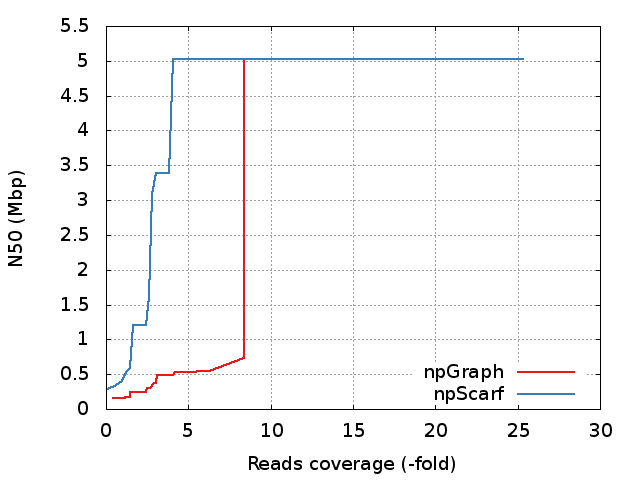
\includegraphics[width=.45\textwidth]{images/rt_cf1374.png}
}
\hfill
\subfloat[\emph{Escherichia~coli} K12 MG1655]{
	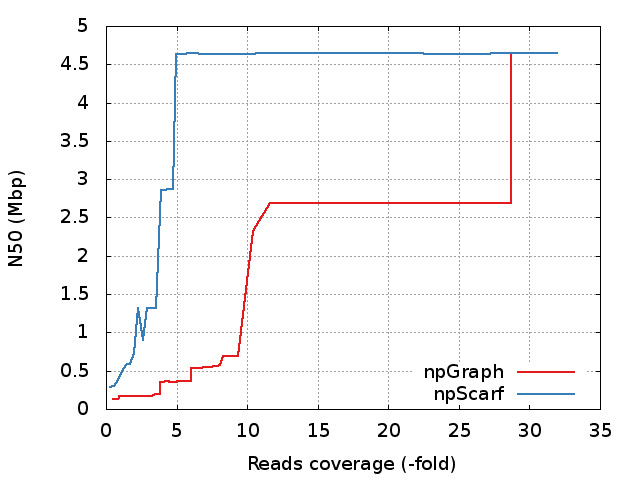
\includegraphics[width=.45\textwidth]{images/rt_eck12.png}
}
\\
\subfloat[\emph{Klebsiella} 30660 NJST258]{
	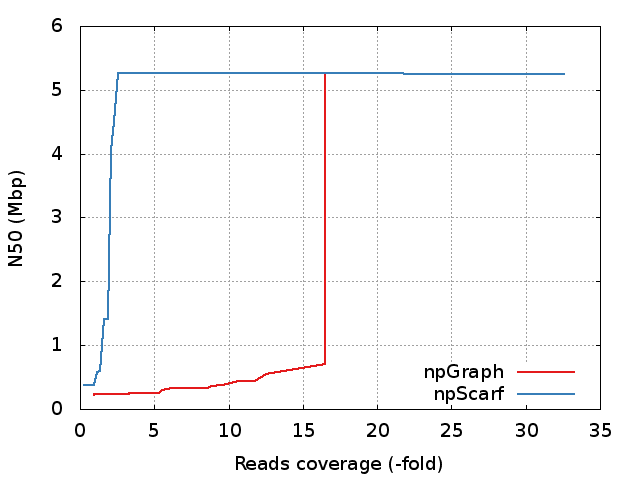
\includegraphics[width=.45\textwidth]{images/rt_kp30660.png}
}
\hfill
\subfloat[\emph{Klebsiella} NTUH K2044]{
	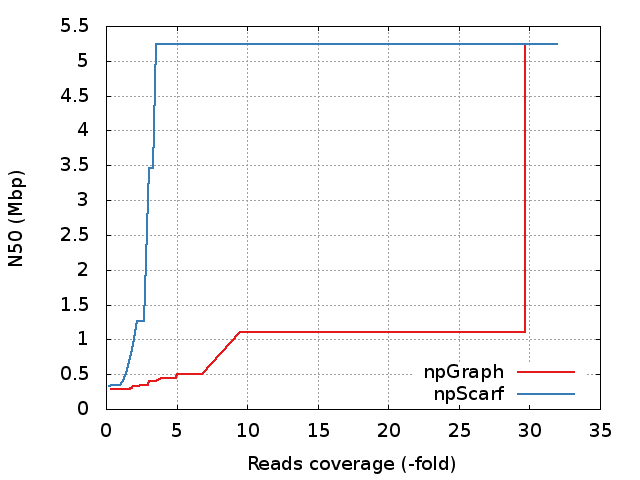
\includegraphics[width=.45\textwidth]{images/rt_kpntuh.png}
}
\caption[Real-time assembly by \npscarf{} and \npgraph{}]{N50 statistics of real-time assembly by \npscarf{} and \npgraph{}.}
\label{F:npgraph_rt}
\end{figure}

As can be observed from all the plots, \npgraph{} and \npscarf{} both converged to the same ultimate completeness but with different paces and patterns.
Apparently it took more data for \npgraph{} to finish the same genome than the other.
The reason stems from the fact that the new algorithm used a more `conservative' approach of bridge construction with at least 3 supporting long-reads for each to prevent any potential mis-assembly. 
Unlike \npscarf{} when the connections could be undone and rectified later if needed, a bridge in \npgraph{} will remain unchanged once created.
The plot for \ec{} data clarifies this behaviour when a fluctuation can be observed in \npscarf{} assembly at $\simeq 3$-folds data coverage.
On the other hand, the N50 length of \npgraph{} is always a monotonic increasing function. 
The sharp \emph{jumping} patterns suggested that the linking information from long-read data had been stored and exploited at certain time point decided by the algorithm. 
In addition, at the end of the streaming when the sequencing is finished, \npgraph{} will try for the last time to connect bridges with less than 3 supporting reads but seeing no conflict until then.

Once a unique path has been determined, the bridge can be formed to connect the fragments together into a longer sequence leading to the increase of N50. \npgraph{} shows stable results so that it can directly report final assembly at any timepoint. As can be seen from Figure~\ref{F:npgraph_rt}, the genomes were completed at slower speed at the beginning of the streaming process and faster toward the end due to the accumulation of bridging information. 
However, the plots here only depict the real-time assembly operation including one final post-processing step. If the process is stopped somewhere in the middle, the post-processing would be invoked to return more completed genome but with the risk of higher mis-assembly due to shortage of supporting data.

%\subsection*{Metagenomics assembly on mock community}
%Here, we ran \npgraph{} on mock community data to study the performance of our method in metagenomic co-assembly problem.
%In this application, sequencing data (including both short and long reads) from mixtures of ten microbial species of ZymoBIOMICS Microbial Community Standards \cite{Nick2019zymo} were used as input for \npgraph{}. 
%The total genome size was estimated as 61.96 Mbp.
%There were two settings for the input depending on the distribution of cell abundances in the mixture itself, namely even and log population.
%On the other hand, 8 out of 10 genomes being sequenced were reconstructed by using PacBio sequencing (RSII and Sequel) previously \cite{Mcintyre2019zymo}, including \emph{Bacillus~subtills}, \emph{Enterococcus~faecalis}, \emph{Escherichia~coli}, \emph{Listeria~monocytogenes}, \emph{Pseudomonas~aeruginosa}, \emph{Saccharomyces~cerevisiae}, \emph{Salmonella~enterica} and \emph{Staphylococcus~aureus}. We evaluated the coassembly results by running $\mathtt{metaQUAST}$ given 8 PacBio assembly as references.
%
%\begin{table}[!hpt]
%\begin{center}
%\caption{Assembly improvement, in terms of NGA50 statistics, from $\mathtt{metaSPAdes}$ to \npgraph{} contigs on two mock communities ZymoLog and ZymoEven \cite{Nick2019zymo}. The statistics were generated by $\mathtt{metaQUAST}$ v3.2 with 8 (out of 10) available PacBio isolate assemblies used as reference \cite{Mcintyre2019zymo}.}
%\label{table:zymo}
%\begin{tabular}{|l|c|r|r|c|r|r|}
%\hline
%\multirow{3}{*}{\textbf{Community}} & \multicolumn{3}{|c|}{\textbf{ZymoEven}} & \multicolumn{3}{|c|}{\textbf{ZymoLog}} \\ \cline{2-7}
%& \multirow{2}{*}{Abundance(\%)} & \multicolumn{2}{|c|}{NGA50} & \multirow{2}{*}{Abundance(\%)} & \multicolumn{2}{|c|}{NGA50} \\ \cline{3-4} \cline{6-7}
%& & $\mathtt{metaSPAdes}$ & \npgraph{} &  & $\mathtt{metaSPAdes}$ & \npgraph{} \\
%\hline
%\emph{L.~monocytogenes} & 12 & $26,480$ & $520,012$ & 89.1 & $23,146$ & $130,284$ \\ \hline
%\emph{P.~aeruginosa} & 12 & $59,372$ & $1,753,658$ & 8.9 & $161,816$ & $444,495$ \\ \hline
%\emph{B.~subtilis} & 12 & $23,386$ & $382,368$ & 0.89 & $35,390$ & $433,078$ \\ \hline
%\emph{S.~cerevisiae} & 2 & $-$ & $-$ & 0.89 & $-$ & $-$ \\ \hline
%\emph{E.~coli} & 12 & $34,776$ & $1,108,989$ & 0.089 & $-$ & $-$ \\ \hline
%\emph{S.~enterica} & 12 & $33,363$ & $4,242,458$ & 0.089 & $-$ & $-$ \\ \hline
%\emph{E.~faecalis} & 12 & $23,340$ & $217,908$ & 0.00089 & $-$ & $-$ \\ \hline
%\emph{S.~aureus} & 12 & $26,058$ & $175,908$ & 0.000089 & $-$ &$-$ \\ \hline
%\end{tabular}
%\end{center}
%\end{table}
%
%To run \npgraph{} on the metagenomics data set, we firstly augmented binning information from using $\mathtt{metaBAT}$ \cite{Kang2015metabat} on the Illumina raw reads, before applying our method to the assembly graph generated by $\mathtt{metaSPAdes}$. The default parameter setting was remained as it was for isolate assembly. 
%
%In terms of Illumina data, Even community had been sequenced by MiSeq platform which generated about 43-fold coverage while the Log community`s short-read data had been obtained from an Illumina HiSeq 1500, for about 156X coverage.
%Even though the total amount of base coverage from the latter was almost four-times richer than the former, its $\mathtt{metaSPAdes}$ assembly quality was lesser. This happened due to the fact of under-presented microbial cells from rare species in the Log population that require much more input for their reads to be sequenced, resulting in significant smaller size of assembly contigs and more fragmented assembly graph (Supplementary Figure~\ref{supp_fig:npgraph_zymo}).
%The assembly size for the two population are approximately 41 Mbp (66\%) and 22 Mbp (36\%). 
%During pre-processing step, \npgraph{} disregarded nodes which represent short, unconnected and extremely-low-coverage contigs which were indistinguishable from sequencing errors, artifacts or the actual rare species` genomes without additional works.
%
%Despite of the input graph quality, table~\ref{table:zymo} shows the assembly improvement in terms of NGA50 after running \npgraph{} on the $\mathtt{metaSPAdes}$' initial graph.  
%As expected from better quality assembly graph, the results for the Even community indicated significant more complete genomes recovered. 
%There were 7 isolate genomes had been identified for this community, compared to only 3 from the more complicated log population.
%\npgraph{} had been able to resolve the assembly graph efficiently for Even community, with the maximum NGA50 improvement for \emph{S.~enterica} boosted from $33$ Kbp to $4.2$ Mbp. 
%On the other hand, genomes from the Log community witnessed increasing length of aligned contigs as well, but not as distinct as for the balanced colony. The longest NGA50 contigs belongs to \emph{P.aeruginosa} of 445 Kbp, however, the counterpart from the Even community was 4-fold than that, at 1.75 Mbp.
%The only exception was \emph{B.~subtilis}, where \npgraph{} can only resolved 382 Kbp correct length from the zymo even while the respective statistics was 433 Kbp for the zymo log. However for this isolate, the initial $\mathtt{metaSPAdes}$ assembly of the former was slightly better compared to the latter`s.
%
%%how much nanopore needed indeed

%%%%%%%%%%%%%%%%%%%%%%%%%%%%%%%%%%%%%%%%%%%%%%%%%%%%%%%%%%%%%%%%%%%%%%%%%%%%%%%%%%%
\section*{Conclusion}
%npgraph: how important hybrid assembly
Due to the limits of current sequencing technology, application of hybrid methods should remain a common practice in whole genome assembly for the near future.
On the other hand, the ONT platforms are evolving quickly with significant improvement in terms of data accuracy and yield, however, the sequencing cost per base is still high. Beside, the real-time property of this technology has not been sufficiently exploited to match its potential benefits.
\npscarf{} had been introduced initially to address these issues, however, the accuracy of the assembly output was affected by its greedy alignment-based scaffolding approach.
Here we present \npgraph{}, a streaming hybrid assembly method working on the DBG assembly graph that is able to finish short-read assembly in real-time while minimizing the errors and mis-assemblies drastically.

Compared to \npscarf, \npgraph{} algorithm employs a less greedy approach based on graph traversal. This might reduce the bridging rate when the linking conditions become more strict, but the concurrent results reported are more reliable.
The performance of \npgraph{} is comparable to \unicycler{} while consuming much less computational resources so that it can work on streaming mode. 
Also, the integrated GUI allows users to visualize its animated output in a  more efficient way.

%In the very first attempt to run real-time assembly on metagenomics data, \npgraph{} proved that its method can adapt to scaled-up data and complexity. The assembler was able to handle the De Bruijin assembly graph from Illumina data generated by $\mathtt{metaSPAdes}$ and simplify it using a minimal input stream of long reads. 
%The result has shown more complete isolate genomes reconstructed out of the graph, but the overall communities` genome coverage were dropped with several strains omitted comparing to the reference. The issue is caused by the shortage of short-read sequencing input to cover underpresented species in the mixture, especially for the Log community.

As a hybrid assembler, similar to \unicycler{}, \npgraph{} relies on the initial assembly graph to generate the final assembly. The algorithm operates on the assumption of a high quality assembly from a well-supplied source of short-read data for a decent assembly graph to begin with.
It then consumes a just-enought amount of data from a streaming input of nanopore reads to resolve the graph. 
Finally, extra pre-processing and comprehensive binning on the initial graph could further improve the performance of the streaming assembler.


%%%%%%%%%%%%%%%%%%%%%%%%%%%%%%%%%%%%%%%%%%%%%%%%%%%%%%%%%%%%%%%%%%%%%%%%%%%%%%%%%%%
\section*{Methods}

The work flow of \npgraph{} mainly consists of 3 stages: (1) assembly graph preprocessing; (2) graph resolving and simplifying; (3) postprocessing and reporting results. 
The first step is to load the graph of Illumina contigs and retrieve their metadata which are helpful for the next steps, \EG binning and multiplicity estimation.
The second step works on the processed input and augmented information from the previous one. In combination with path inducing from long reads, the assembly graph is then traversed and resolved in real-time.
Finally, the graph is subjected to the last attempt of resolving and cleaning, as well as output the final results. The whole process can be managed by using either command-line interface or GUI.
Among three phases, only the first one must be performed prior to the MinION sequencing process in a streaming setup.
The algorithm works on the assembly graph of Illumina contigs, so the terms \emph{contigs} and \emph{nodes} if not mentioned specifically, would be used interchangable throughout this context.
\subsection*{Contigs binning}
Contigs from each completed genome are expected to be assigned to an unique group, or \emph{bin}, that would represent the final assembly unit, \EG{} chromosome , plasmids, or even particular species genome in a metagenomic community. As a result, the binning phase would assist the multiplicity estimation submodule that can differentiate repetitive contigs from unique ones. 

Each contig is embeded in a single node in the assembly graph and an edge between two nodes indicates their overlap (link) properties.
This step is to cluster the biggest nodes (contigs longer than $10$Kbp) into different sets, namely \emph{core} groups, based on the their degree (number of connections) and coverage values.
DBSCAN clustering algorithm \cite{Ester96adensity-based} is applied for this task by default.
The rationale is to approximate a coverage value of an extremely long contig (which can be splitted into more than 10,000 \emph{k-mers}) to be a sampled mean of a Poisson distribution (of \emph{k-mers} count). 
The metric is a distance function based on Kullback-Leibner divergence \cite{Kullback1951information}, or relative entropy, of two Poisson distributions. 

Assuming there are 2 Poisson distributions $P_1$ and $P_2$ with density functions $$p_1(x,\lambda_1)=\frac{e^{-\lambda_1}\lambda_1^x}{\Gamma(x+1)}$$ and $$p_2(x,\lambda_2)=\frac{e^{-\lambda_2}\lambda_2^x}{\Gamma(x+1)}$$ 
The Kullback-Leibner divergence from $P_2$ to $P_1$ is defined as:
$$D_{KL}(P_1||P_2)=\int_{-\infty}^{\infty} p_1(x)\log{\frac{p_1(x)}{p_2(x)}} dx$$
or in other words,  it is the expectation of the logarithmic difference between the probabilities $P_1$ and $P_2$, where the expectation is taken with regard to $P_1$.
The log ratio of the density functions is
$$\log{\frac{p_1(x)}{p_2(x)}}=x\log{\frac{\lambda_1}{\lambda_2}}+\lambda_2-\lambda_1$$
take expectation of this expression with regard to $P_1$ with mean $\lambda_1$ we have
$$D_{KL}(P_1||P_2)=\lambda_1\log{\frac{\lambda_1}{\lambda_2}}+\lambda_2-\lambda_1$$
The metric we used is the distance defined as
$$D(P_1,P_2)=\frac{D_{KL}(P_1||P_2)+D_{KL}(P_2||P_1)}{2}=\frac{1}{2}(\lambda_1-\lambda_2)(\log{\lambda_1}-\log{\lambda_2})$$

We implemented a simple binning algorithm based on the clustered contigs, the graph topology as well as statistics calculated by length and coverage of each contigs. 
Additional binning step is taken place in real-time using the long reads as well. In this context, the repetition or uniquess of ambigous nodes are determined with sufficient supporting evidence from the long-spanning reads.
Generally, the algorithm performs well for isolate or simple simulated metagenomics, but ineffective for complicated community. In that case, external binning tools can be employed for more comprehensive binning task and the results can be augmented to \npgraph{} input.
If external binning algorithm is employed, the resulting output must be converted into a text file that specifies the corresponding bin of every contigs, just like output from MetaBAT. By that, each line of the file would be:
$
\mathtt{<contig\_ID>} \; ~ \mathtt{<bin\_ID>}
$
where $\mathtt{bin\_ID}=0$ indicates unspecified binned contigs.
\subsection*{Multiplicity estimation}
Due to the possible divergence of sequencing coverage relative to the real abundance of sequences, especially for the shorter contigs, an optimization step is carried out to alleviate this issue.
The re-estimation is basically carried out by following two steps.
\begin{itemize}
\item[1.] From nodes coverage, estimate edges' value by quadratic unconstrained optimization of the least-square function:
$$\frac{1}{2}\sum_{i}{l_i((\sum{e^{+}_{i}}-c_i)^2+(\sum{e^{-}_{i}}-c_i)^2}$$
where $l_i$ and $c_i$ is the length and coverage of a node $i$ in the graph;

$\sum{e^{+}_{i}}$ and $\sum{e^{-}_{i}}$ indicates sum of the values of incoming and outgoing edges from $i$ respectively. 
The above function and be rewritten as:
$$f(x)=\frac{1}{2}x^TQx + b^Tx + r$$
and then being minimized by using gradient-based method.
\item[2.] Update nodes' coverage based on itself and its neighbor edges' measures.
\end{itemize}
The calibration is iterative until no further improvements are made or a threshold loop count is reached.
The coverage measures of nodes (which represent contigs) are propated throughout the graph via connecting edges for calibrations prior to the multiplicity estimation. 
%The assignment of coverage to edges is also helpful to induce multiplicity of nodes in later step. 

Based on the coverage values of all the edges and the graph's topology, we induce the copy numbers of every significant nodes (long contigs) in the final paths.
For each node, this could be done by investigating its adjacent edges and answering the questions of how many times it should be visited, from which abundance groups.
Multiplicities of insignificant nodes (of sequences with length less than $1,000$ bp) can be estimated in the same way but usually with less confident due to more complicated connections and greater variation of coverage values. 
For that reason, in \npgraph{}'s algorithm, they are only used as augmented information to calculate likelihood scores of candidate paths containing corresponding nodes.

%\subsection*{Untangling assembly graph by stream of nanopore data.}
\subsection*{Building bridges in real-time}
Bridge is the data structure designed for tracking the possible connections between two anchored nodes (of unique contigs) in the assembly graph.
A bridge must start from a unique contig, or \emph{anchor} node, and end at another when completed. Located inbetween are nodes known as \emph{steps} and distances between them are called \emph{spans} of the bridge. Stepping nodes are normally repetitive contigs and indicative for a path finding operation later on. In a complicated assembly graph, the more details the bridge, \emph{a.k.a.} more steps inbetween, the faster and more accurate the linking path it would resolve. A bridge's function is complete when it successfully return the ultimate linking path between 2 anchors.

The real-time bridging method considers the dynamic aspect of multiplicity measures for each node, meaning that a $n$-times repetitive node might become a unique node at certain time point when its $(n-1)$ occurrences have been already identified in other distinct unique paths. 
Furthermore, the streaming fashion of this method allows the bridge constructions (updating steps and spans) to be carried out progressively so that assembly decisions can be made immediately after having sufficient supporting data.
A bridge in \npgraph{} has several completion levels. When created, it must be rooted from an \emph{anchor node} which represents a unique contig (level 1). A bridge is known as fully complete (level 4) if and only if there is a unique path connecting its two anchor nodes from two ends. 

\begin{figure}[!hpt]
\centering
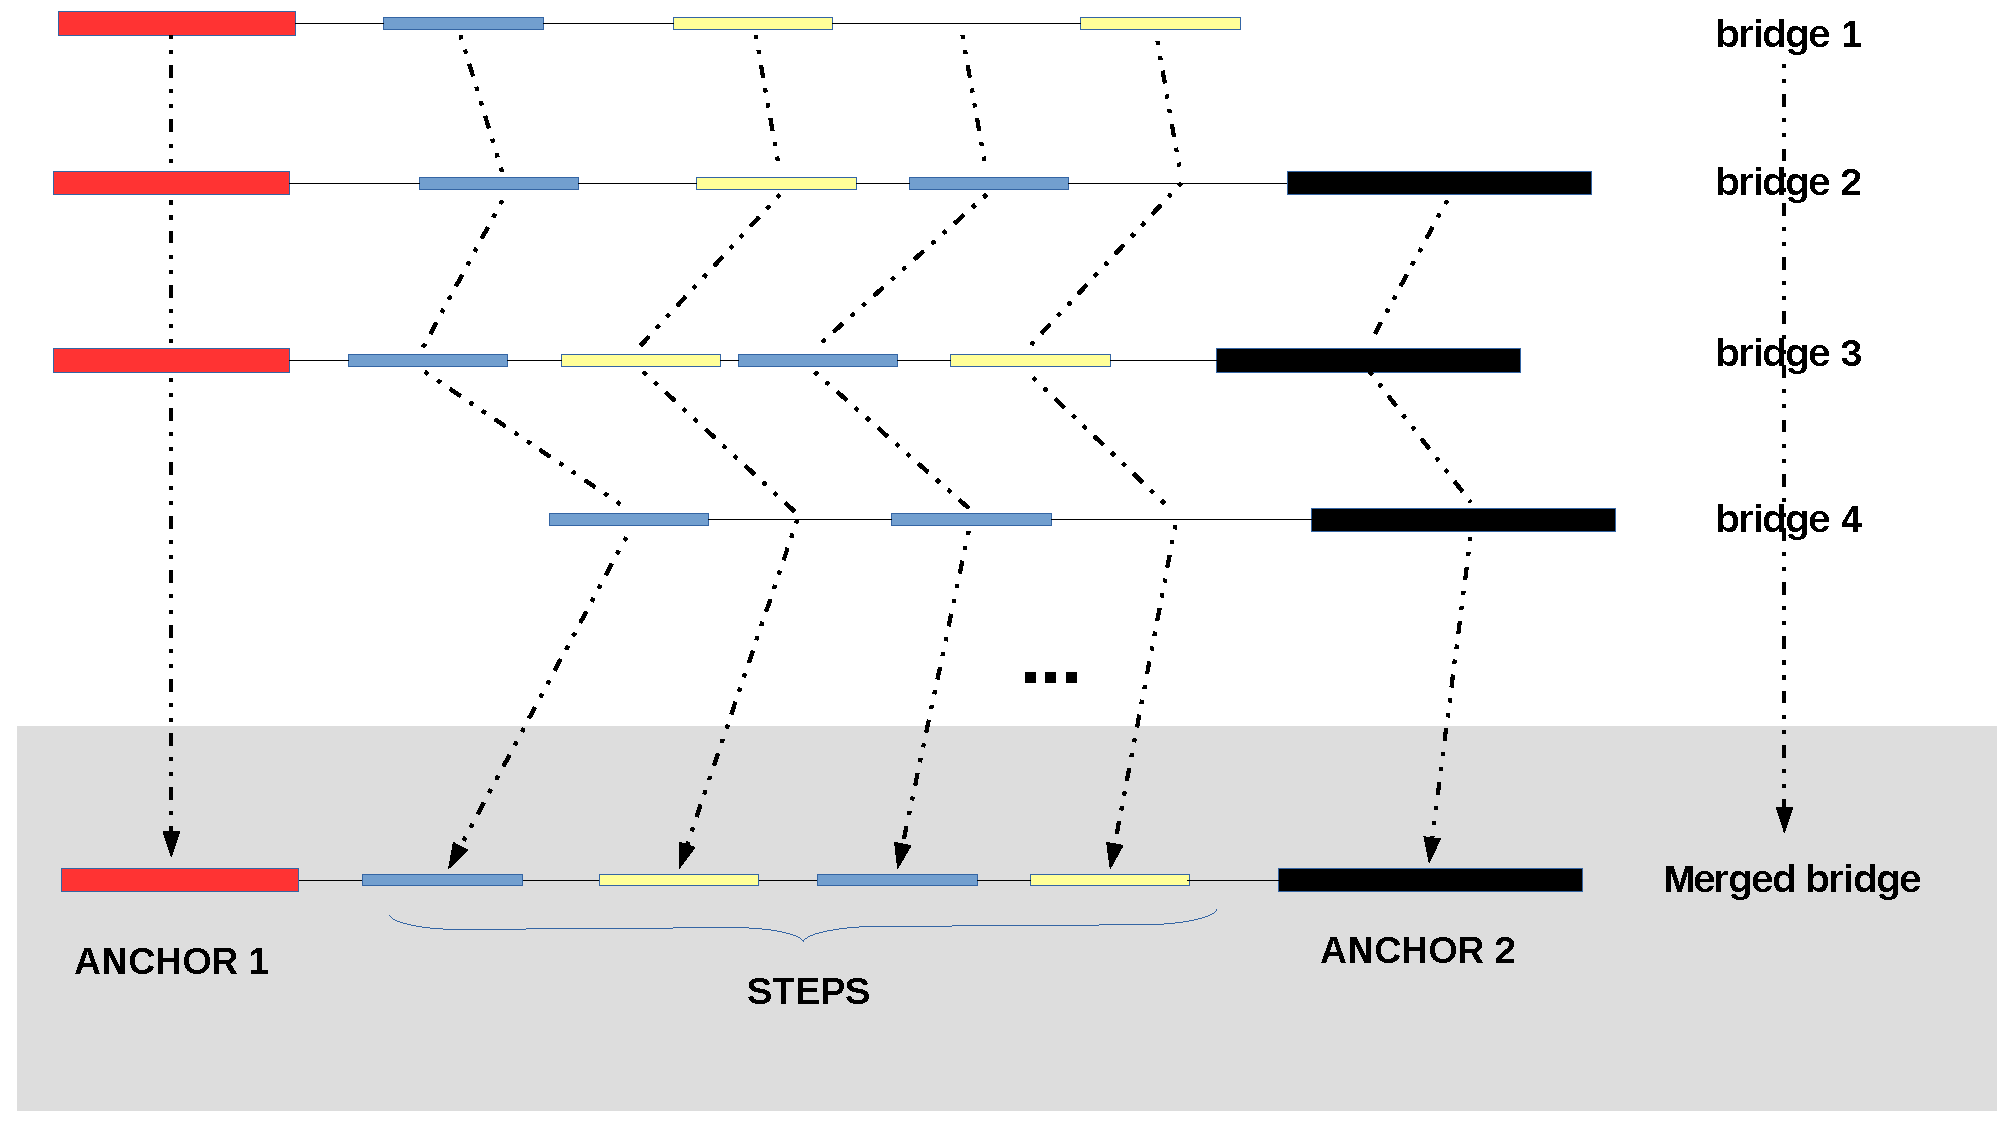
\includegraphics[width=.8\textwidth]{images/bridge_merging.pdf}
\caption[Example of bridge merging progressively]{Bridge merging progressively in real-time. Sequencing long reads induce alignments to the contigs where new bridges are created respectively. Bridges sharing same anchors can be merged together to form the ultimate, more comprehensive bridge (with more step nodes and better approximation of spans between them).}
\label{figure:npgraph_merging}
\end{figure}

At early stages (level 1 or 2), a bridge is constructed progressively by alignments from long reads that spanning its corresponding anchor(s).
In an example from Figure~\ref{figure:npgraph_merging}, bridges from a certain anchor (highlighted in red) are created by extracting appropriate alignments from incoming long reads to the contigs. Each of the steps therefore is assigned a weighing score based on its alignment quality.
Due to the error rate of long reads, there should be deviations in terms of steps found and spans measured between these bridges, eventhough they represent the same connection.
A continuous merging phase, as shown in the figure, takes advantage of a pairwise Needleman-Wunsch dynamic programming to generate a consensus list based on weight and position of each of every stepping nodes. The spans are calibrated accordingly by averaging out the distances. On the other hand, the score of the merged steps are accumulated over time as well.
Whenever a consensus bridge is anchored by 2 unique contigs at both ends and hosting a list of steps with sufficient coverage, it is ready for a path finding in the next step.


\subsection*{Path finding algorithm}
Given a bridge with 2 anchors, a path finding algorithm is invoked to find all candidate paths between them. Each of these paths is given a score of alignment-based likelihood which are updated immediately as long as there is an appropriate long read being generated by the sequencer. As more nanopore data arrives, the divergence between candidates' score becomes greater and only the top-scored ones are kept for the next round.
We implement a modified stack-based version utilizing Dijkstra's shortest path finding algorithm~\cite{Dijkstra1959} to reduce the search space when using Depth-First Search.

Due to false alignments from shorter contigs to the long reads, not all of the reported step nodes are neccessary to be appeared in the ultimate path resolved by the bridge. 
In most cases, the accumulated score of each step indicates its likelihood to be the true component of the final solution.
For that reason, a strategy similar to binary searching is employed to find a path across 2 anchors of a bridge as shown in Algorithm~\ref{algo:binsearch}.


Before that, we define Algorithm~\ref{algo:findpath} to demonstrates the path finding algorithm for two nodes given their estimated distance. In which, function 
$\mathtt{shortestTree}(\overrightarrow{vertex},distance) : (V,Z) \rightarrow V^n$ 
from line 3 of the algorithm's pseudo code builds a shortest tree rooted from $\overrightarrow{v}$, following its direction until a distance of approximately $d$ (with a tolerance regarding nanopore read error rate) is reached. This task is implemented based on Dijkstra algorithm.
This tree is used on line 4 and in function $includedIn()$ on line 19 to filter out any node or edge with ending nodes that do not belong to the tree.

\begin{algorithm}[!hpt]
\DontPrintSemicolon
\KwData{Assembly graph $G\{V,E\}$}
\KwIn{Pair of bidirected nodes $\overrightarrow{v_1}, \overrightarrow{v_2}$ and estimated distance $d$ between them}
\KwOut{Set of candidate paths connecting $\overrightarrow{v_1}$ to $\overrightarrow{v_2}$ with reasonable distances compared to $d$}
\SetKwFunction{DFS}{DFS} 
\SetKwProg{Fn}{Function}{:}{}
\Fn{\DFS{$\overrightarrow{v_1}, \overrightarrow{v_2}$, $d$}}{
$P$:=new List()\;
$M$:=$\mathtt{shortestTree}(\overrightarrow{v_2},d)$ \tcp*{build shortest tree from $\overrightarrow{v_2}$ with range $d$}
\If{$M.contain(\overrightarrow{v_1})$}{
    $S$:=new $Stack()$ \tcp*{stack of sets of edges to traverse}
    $edgesSet$:=$getEdges(\overrightarrow{v_1})$ \tcp*{get all bidirected edges going from $\overrightarrow{v_1}$}
    $S.push(edgesSet)$\;
    $p$:=new $Path(\overrightarrow{v_1})$ \tcp*{init a path that has $\overrightarrow{v_1}$ as root}
    \While{true}{
        $edgesSet$:=$S.peek()$\;
        \If{$edgesSet.isEmpty()$}{
            \If{$p.size() \leq 1$}{
                $\mathbf{break}$ \tcp*{stop the loop when there is no more edge to discover}
            }
        $S.pop()$\;
        $d$+=$p.peekNode.length()+p.popEdge().length()$\; 
        }
        \Else{
            $curEdge \coloneqq edgesSet.remove()$\;
            $\overrightarrow{v}$:=$curEdge.getOpposite(p.peekNode())$\;
            $S.push(getEdges(\overrightarrow{v}).includedIn(M))$\;
            $p.add(curEdge)$\;
            \If{reach $\overrightarrow{v_2}$ with reasonable $d$}{
                $P.add(p)$\;
            }
            $d$-=$\overrightarrow{v}.length()+curEdge.length()$\;
        }
    }
}

\Return{$P$}
}
\caption{Pseudo-code for finding paths connecting 2 nodes given their estimated distance.}
\label{algo:findpath}
\end{algorithm}

\begin{algorithm}[!hpt]
\DontPrintSemicolon
\KwData{Assembly graph $G\{V,E\}$}
\KwIn{Brigde $B:\lbrace\overrightarrow{v_0}, ...\overrightarrow{v_k}, ...,\overrightarrow{v_n}\rbrace$ with $\overrightarrow{v_0}$ and $\overrightarrow{v_n}$ are two anchors, $\{\overrightarrow{v_k}\}, k=1\ldots(n-1)$ are steps inbetween}
\KwOut{Set of candidate paths connecting $\overrightarrow{v_0}$ to $\overrightarrow{v_2}$ that maximize the likelihood of the step list.}
\SetKwFunction{BinaryBridging}{BinaryBridging} 
\SetKwProg{Fn}{Function}{:}{}
\Fn{\BinaryBridging{B}}{
\tcc{search for the contig with maximum score from the step list (two ends excluded)}
$m$:=$\argmax_k(\overrightarrow{v_k}.score())$ \;
\tcc{if there is no step inbetween, run path finding algorithm above directly and return the result}
\If{$M.size() \equiv 2$}{ 
	\Return{$\mathtt{DFS}(B.start(),B.end().B.distance())$}
}
\tcc{divide the original bridge $B$ into 2 bridges by $v_m$: $BL$ and $BR$}
$BL$:=$\lbrace B.start(), ...,\overrightarrow{v_m}\rbrace$ \;
$BR$:=$\lbrace \overrightarrow{v_m}, ...,B.end()\rbrace$ \;
\tcc{Return the join of running recursive function on two sub-bridges}
\Return{$\BinaryBridging(BL)\Join\BinaryBridging(BR)$} 
}
\caption{Recursive binary bridging to connect 2 anchor nodes.}
\label{algo:binsearch}
\end{algorithm}

Basically, the algorithm keeps track of a stack that contains sets of candidate edges to discover. During the traversal, a variable $d$ is updated as an estimation for the distance to the target. A hit is reported if the target node is reached with a reasonable distance \IE{} close to zero, within a given tolerance (line 21). 
A threshold for the traversing depth is set (150) to ignore too complicated and time-consuming path searching.

Note that the $length()$ functions for node and edge are totally different. While the former returns the length of the sequence represented by the node, \IE{} contig from short-read assembly, the latter is usually negative because an edge models a link between two nodes, which is normally an overlap (except for composite edges). For example, in a \emph{k-mers} SPAdes assembly graph, the value of an edge is $-k+1$. 

In many cases, due to dead-ends, there not always exist a path in the assembly graph connecting two anchors as suggested by the alignments. In this case, if enough long reads coverage (20X) are met, a consensus module is invoked and the resulting sequence is contained in a \emph{pseudo} edge.
\subsection*{Graph simplification in real-time}
\npgraph{} resolves the graph by reducing its complexity perpetually using the long reads that can be streamed in real-time.
Whenever a bridge is finished (with a unique linking path), the assembly graph is \emph{transformed} or \emph{reduced} by replacing its unique path with a composite edge and removing any unique edges (edges coming from unique nodes) along the path. The assembly graph would have at least one edge less than the original after the reduction. The nodes located on the reduced path, other than 2 ends, also have their multiplicities subtracted by one and the bridge is marked as finally resolved without any further modifications. 

\begin{figure}[!hpt]
\centering
\subfloat[Initial graph]{
	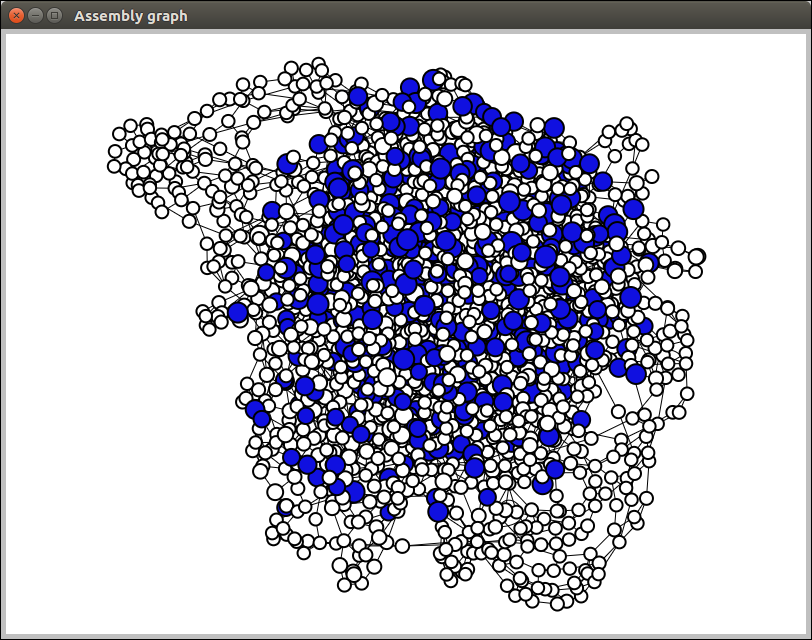
\includegraphics[width=.45\textwidth]{images/npgraph_shigella_0.png}
}
\hfill
\subfloat[Resolved graph]{
	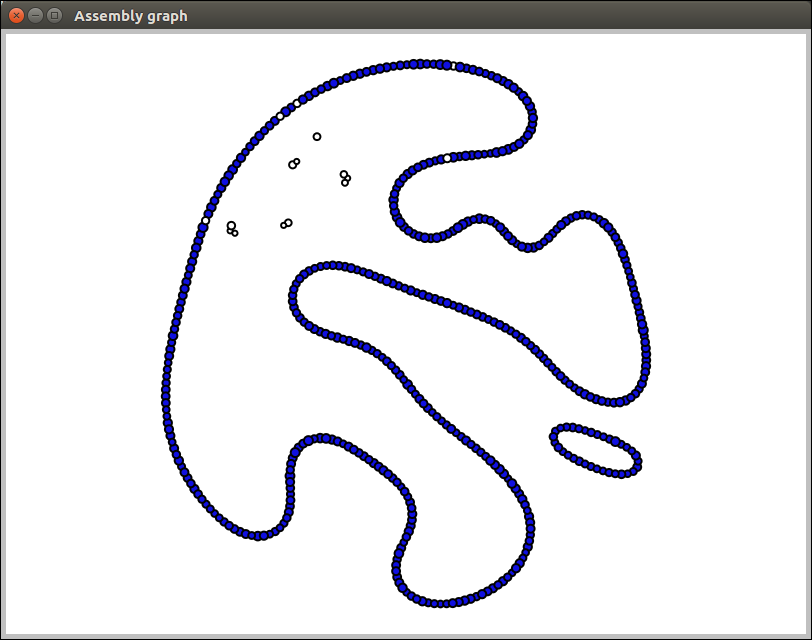
\includegraphics[width=.45\textwidth]{images/npgraph_shigella_2.png}
}
\caption[Assembly graph resolving on \npgraph{} Graph View]{Assembly graph of \emph{Shigella~dysenteriae} Sd197 synthetic data being resolved by \npgraph{} and displayed on the GUI Graph View. The \spades{} assembly graph contains 2186 nodes and 3061 edges, after the assembly shows 2 circular paths representing the chromosome and one plasmid.}
\label{figure:npgraph_graphview}
\end{figure}

Figure~\ref{figure:npgraph_graphview} presents an example of the results before and after graph resolving process in the GUI.
The result graph, after cleaning, would only report the significant connected components that represents the final contigs.
Smaller fragments, even unfinished but with high remaining coverage, are also presented as potential candidates for further downstream analysis.
Further annotation utility can be implemented in the future better monitoring the features of interests as in \npscarf{}.
\subsection*{Result extraction and output}
\npgraph{} reports assembly result in real-time by decomposing the assembly graph into a set of longest straight paths (LSP), each of the LSP will spell a contig in the assembly report.
The final assembly output contains files in both FASTA and GFAv1 format (\url{https://github.com/GFA-spec/GFA-spec}). While the former only retains the actual genome sequences from the final decomposed graph, the latter output file can store almost every properties of the ultimate graph such as nodes, links and potential paths between them.

A path $p=\{v_0,e_1,v_1,\ldots,v_{k-1},e_k,v_k\}$ of size $k$ is considered as straight if and only if each of every edges along the path $e_i, \forall i=1,\ldots,k$ is the only option to traverse from either $v_{i-1}$ or $v_i$, giving the transition rule.
To decompose the graph, the tool simply mask out all incoming/outgoing edges rooted from any node with in/out degree greater than 1 as demonstrated in Figure~\ref{figure:npgraph_decompose}. These edges are defined as branching edges which stop straight paths from further extending.

\begin{figure}[!hpt]
\centering
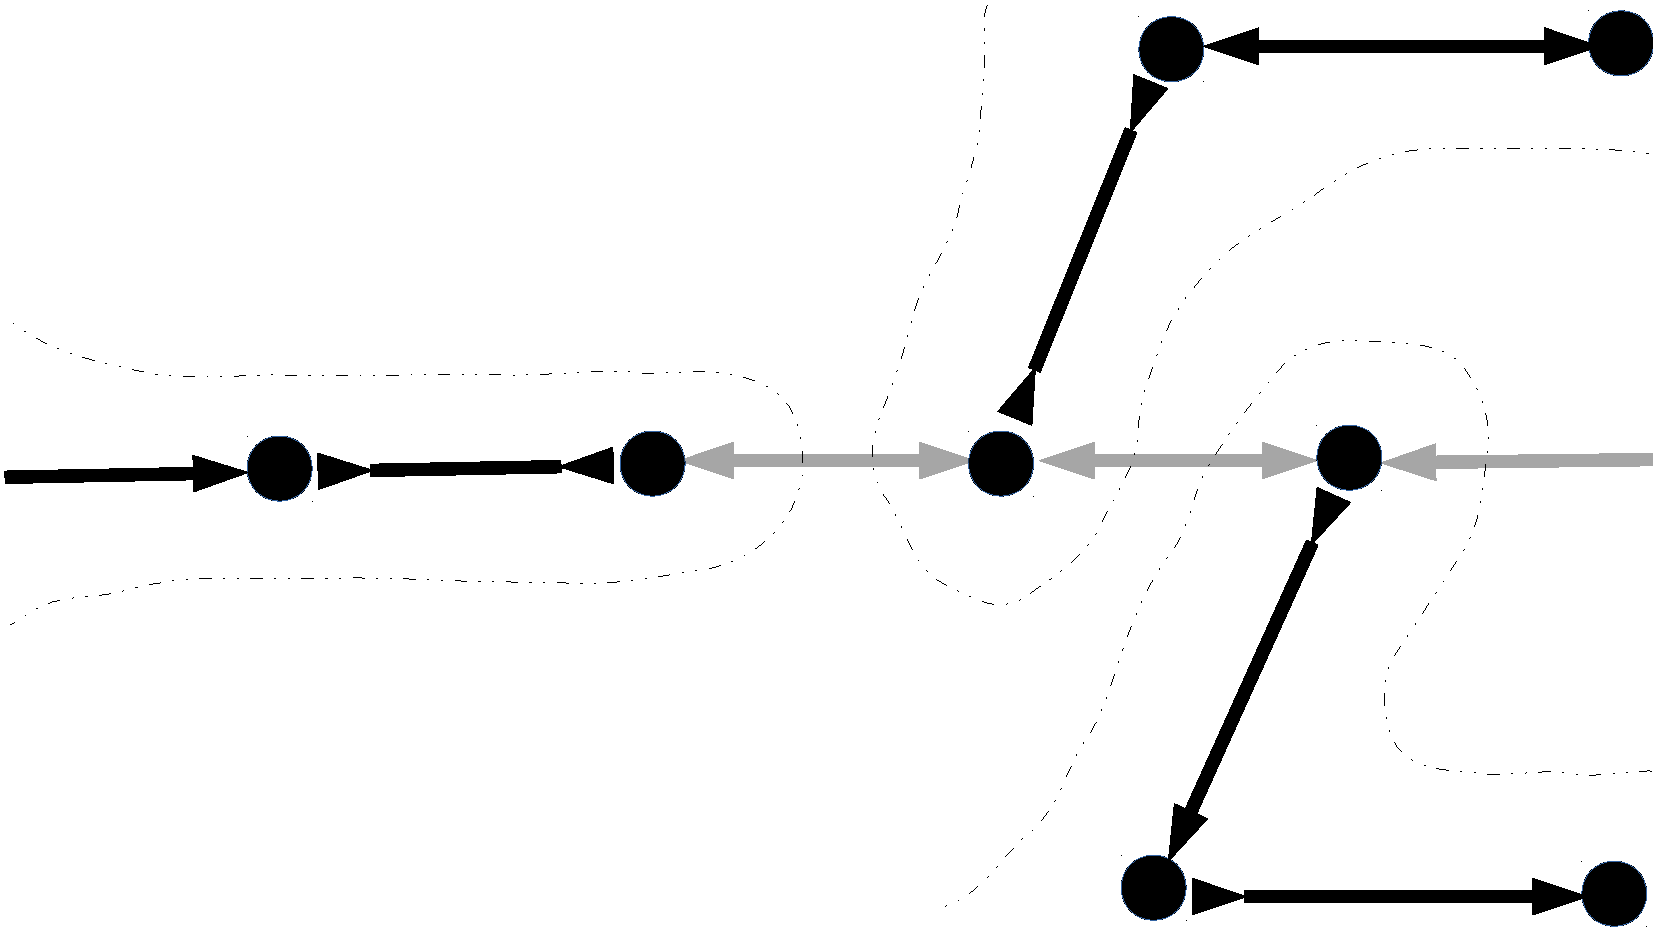
\includegraphics[width=.6\textwidth]{images/decompose.pdf}
\caption[Example of graph decomposition into longest straight paths]{Example of graph decomposition into longest straight paths. Branching edges are masked out (shaded) leaving only straight paths (bold colored) to report. There would be 3 contigs extracted by traversing along the straight paths here.}
\label{figure:npgraph_decompose}
\end{figure}

The decomposed graph is only used to report the contigs that can be extracted from an assembly graph at certain time point. For that reason, the branching edges are only masked but not removed from the original graph as they would be used for further bridging.

Other than that, if GUI mode is enabled, basic assembly statistics such as N50, N75, maximal contigs length, number of contigs can be visually reported to the users in real-time beside the Dashboard. The progressive simplification of the assembly graph can also be observed at the same time in the Graph view.

\bibliographystyle{pnas2011}
\bibliography{library} 

\end{document}
